\subsubsubsection{Scheduling}
The scheduling package contains a pool of worker threads
which consume work items. In our
simulations, each action of an agent corresponds to a work item.

The scheduling system instantiates two executors, one for the travelers and
one for traffic lights.

These two executors are different instances of the same class.
The traffic light executor has a less number of worker threads
than the travelers executor.

We will present our scheduling component by first describing how our system
starts, then how it executes work items and how it stops.
Finally, we will have a quick look at the \texttt{Callback} hierarchy.

\paragraph{Start}

Scheduling is started asynchronously by providing a list of work items
(or \textit{agenda}), which correspond to either travelers' or traffic
lights' actions.
Scheduling will just process this list by registering events at the time
reported in the agenda.

\paragraph{Execution}

In Figure \ref{fig:schedule-execution} we show how a request to schedule
an entity is handled:

\begin{enumerate}
  \item The \texttt{Scheduler} delegates the execution of an action to
    an \texttt{Executor}: the latter is an interface which is implemented by
    the \texttt{SimpleExecutor} concrete class in our system;
  \item \texttt{SimpleExecutor} use the \texttt{Timing} package passing
  the time to defer the action as a parameter. This package
  wraps the executors inside an handler and registers the deferred callback
  in the Ada runtime using the \texttt{Ada.Real\_Time.Timing\_Events} package
  \cite{taft2006ada};
  \item When the timer expires, the Ada scheduler runs the registered handler
  which triggers the \texttt{Executor} reference to
  execute an action (the one originally delegated by the \texttt{Scheduler});
  \item If it is not stopped, \texttt{SimpleExecutor} add this action to the
    \texttt{WorkQueue};
  \item An idle \texttt{WorkerThread}, which was waiting for an item to
    execute, can dequeue the new item from the FIFO \texttt{WorkQueue}
    and consume it.
\end{enumerate}

\begin{figure}[H]
\centering
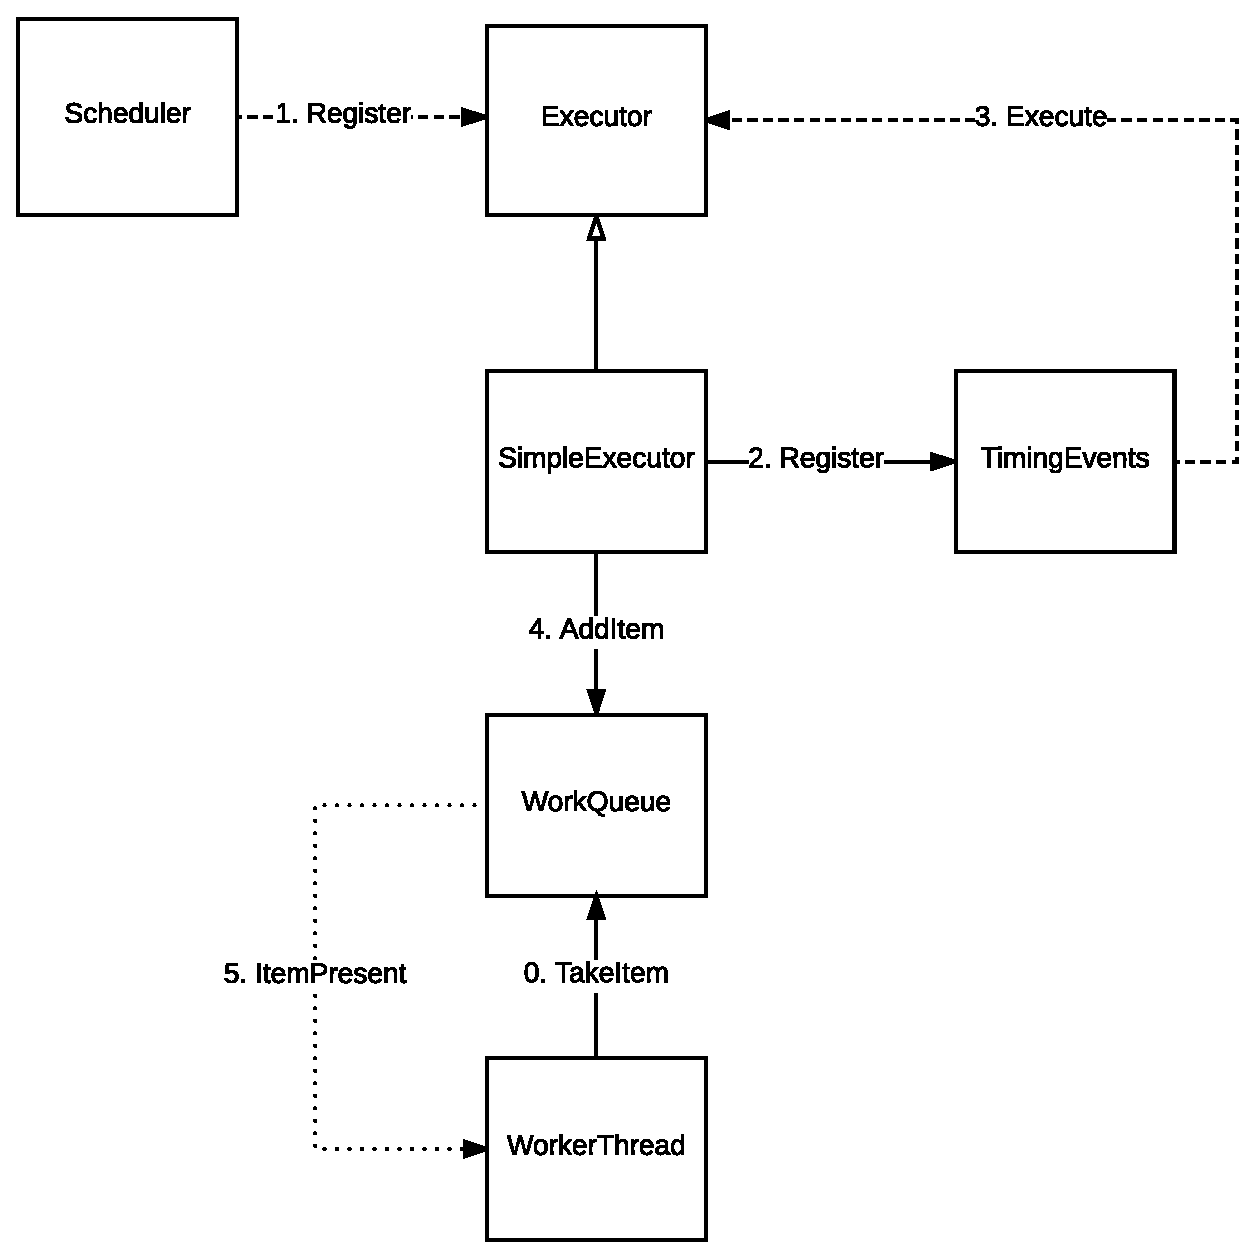
\includegraphics[scale=0.5,keepaspectratio]{images/solution/app/backend/scheduling-execution.eps}
\caption{Execution of a work item}
\label{fig:schedule-execution}
\end{figure}

\paragraph{Termination}

In Figure \ref{fig:schedule-termination} we show how a request to schedule
the termination of an entity is handled:

\begin{enumerate}
  \item The \texttt{Scheduler} asks the \texttt{Executor}s to shutdown;
  \item \texttt{SimpleExecutor} stops itself and then loads in the work queue
    one poison pill for each worker thread of its thread pool;
  \item Eventually, each worker thread will fetch a poison pill from the work
    queue;
  \item When trying to consume a poison pill, a worker thread will stop
    itself on a barrier between it and the Executor;
  \item Finally, when all the workers are stopped, the Executor is unblocked
    from the the barrier.
\end{enumerate}

\begin{figure}[H]
\centering
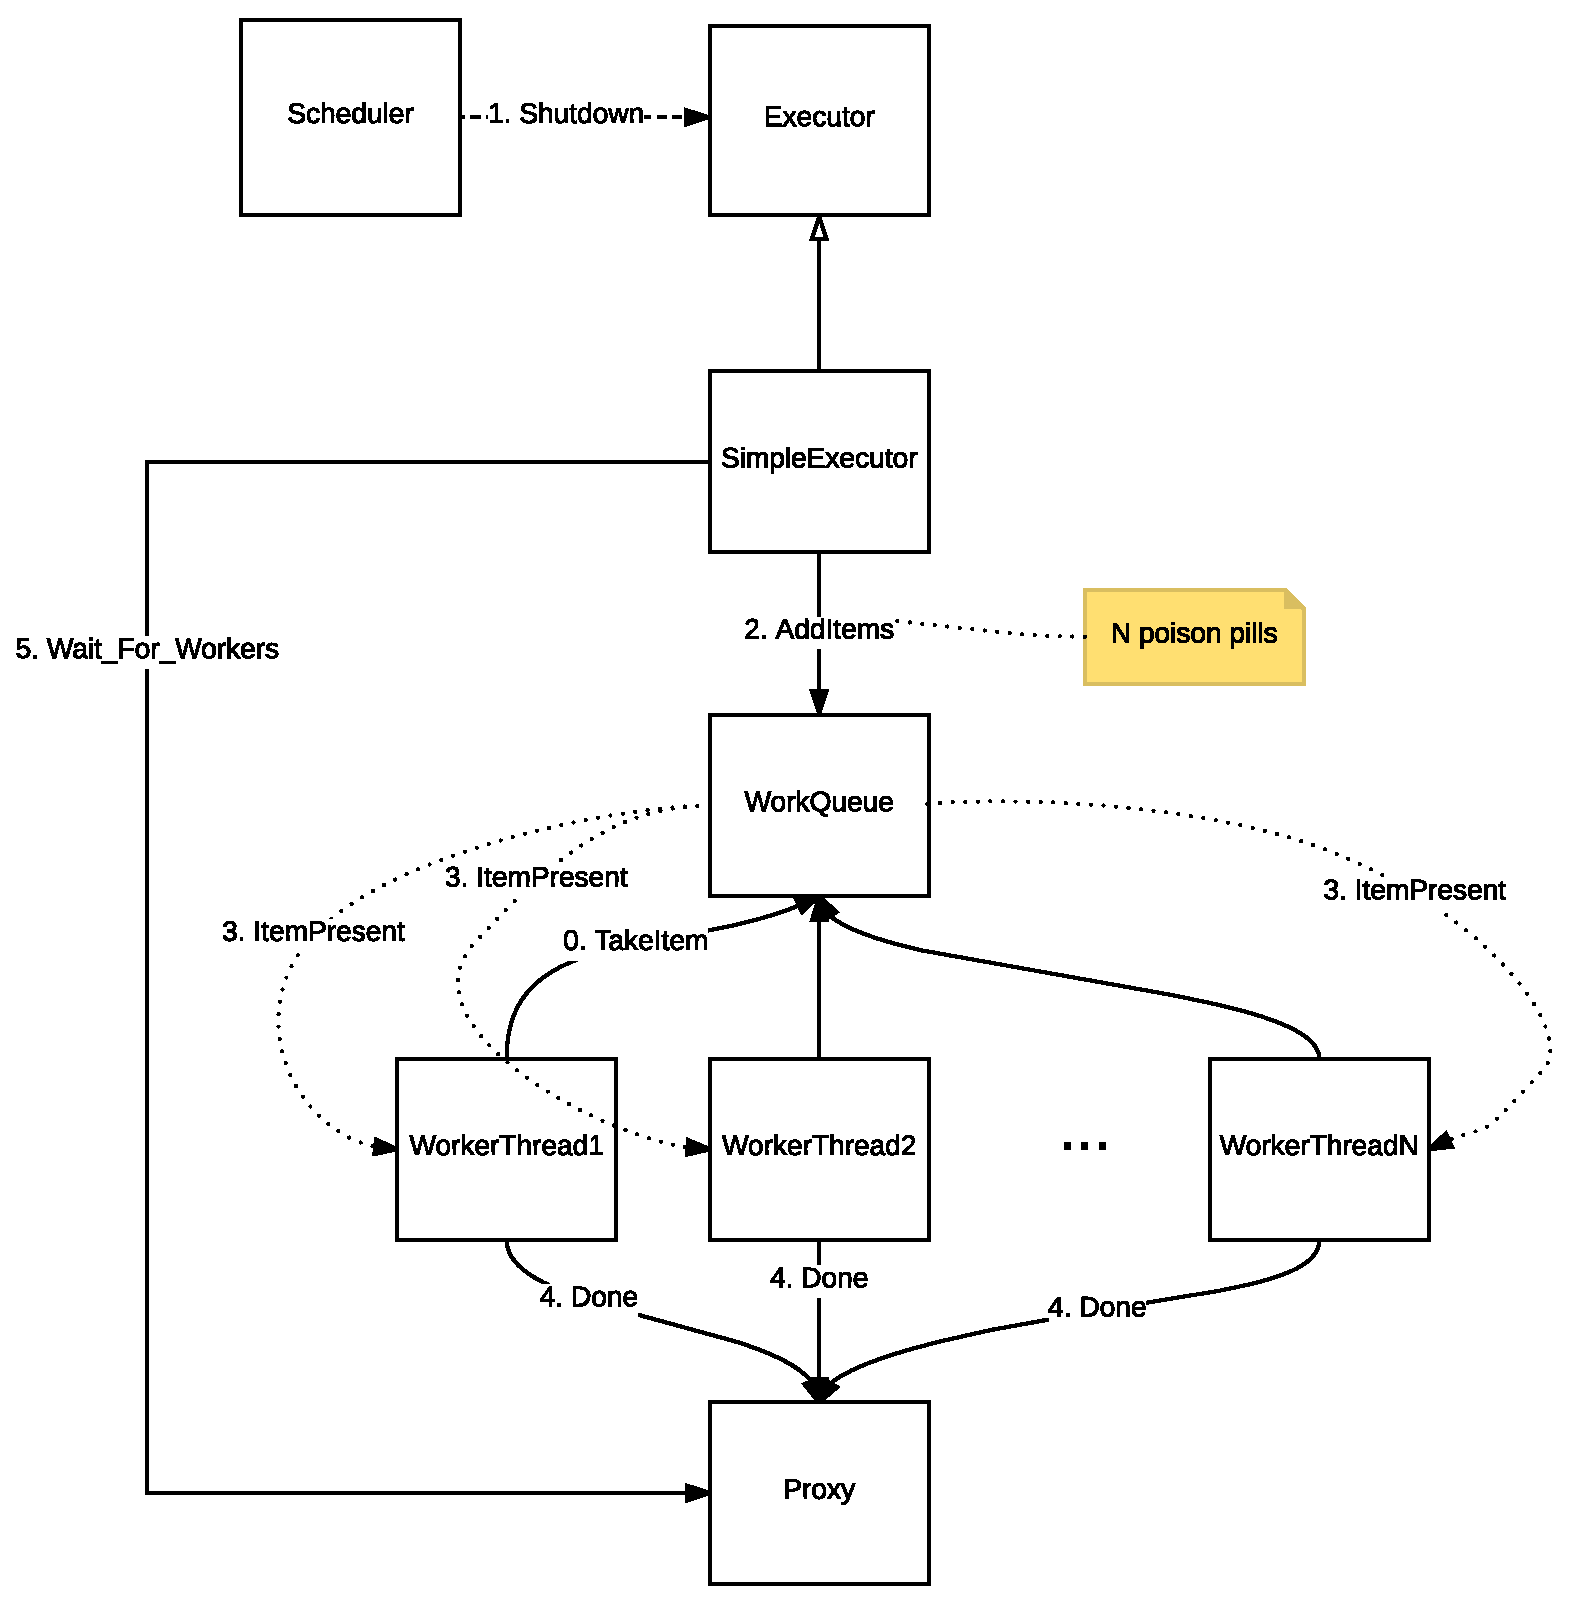
\includegraphics[scale=0.5,keepaspectratio]{images/solution/app/backend/scheduling-termination.eps}
\caption{Scheduling termination}
\label{fig:schedule-termination}
\end{figure}

\paragraph{Callbacks}

As we can see from the code, we implemented four callbacks (actually, two
pairs of success/failure callbacks).
We introduced this mechanism in our system to avoid
communication deadlocks on synchronous remote calls.
Indeed, during some simulation it may happen
that all the worker threads are
blocked on several remote calls which receives no response.
In this case the scheduling system would block and all the agents would not
been scheduled.

Each callback is inserted in a pending requests map
and referenced by the message identifier.
IL is in charge of handling the callbacks inserted in the map based on the
received replies.
